

%%%%%%%%%%%%%%%%%%%%%%%%%%%%%%%%%%%%%%%%%
% University/School Laboratory Report
% LaTeX Template
% Version 3.1 (25/3/14)
%
% This template has been downloaded from:
% http://www.LaTeXTemplates.com
%
% Original author:
% Linux and Unix Users Group at Virginia Tech Wiki 
% (https://vtluug.org/wiki/Example_LaTeX_chem_lab_report)
%
% License:
% CC BY-NC-SA 3.0 (http://creativecommons.org/licenses/by-nc-sa/3.0/)
%
%%%%%%%%%%%%%%%%%%%%%%%%%%%%%%%%%%%%%%%%%

%----------------------------------------------------------------------------------------
%	PACKAGES AND DOCUMENT CONFIGURATIONS
%----------------------------------------------------------------------------------------

\documentclass{article}

\usepackage[version=3]{mhchem} % Package for chemical equation typesetting
\usepackage{siunitx} % Provides the \SI{}{} and \si{} command for typesetting SI units
\usepackage{graphicx} % Required for the inclusion of images
\usepackage{natbib} % Required to change bibliography style to APA
\usepackage{amsmath} % Required for some math elements 
\usepackage{listings}
\usepackage{color}
\usepackage{caption}

\definecolor{dkgreen}{rgb}{0,0.6,0}
\definecolor{gray}{rgb}{0.5,0.5,0.5}
\definecolor{mauve}{rgb}{0.58,0,0.82}

\lstset{frame=tb,
  language=Java,
  aboveskip=3mm,
  belowskip=3mm,
  showstringspaces=false,
  columns=flexible,
  basicstyle={\small\ttfamily},
  numbers=none,
  numberstyle=\tiny\color{gray},
  keywordstyle=\color{blue},
  commentstyle=\color{dkgreen},
  stringstyle=\color{mauve},
  breaklines=true,
  breakatwhitespace=true,
  tabsize=3
}
\setlength\parindent{0pt} % Removes all indentation from paragraphs

\renewcommand{\labelenumi}{\alph{enumi}.} % Make numbering in the enumerate environment by letter rather than number (e.g. section 6)

%\usepackage{times} % Uncomment to use the Times New Roman font

%----------------------------------------------------s------------------------------------
%	DOCUMENT INFORMATION
%----------------------------------------------------------------------------------------

\title{Laboratory Assignment 3 Write Up \\ Computer Science 441} % Title

\author{\textsc{Andreas Bach Landgrebe} \\} % Author name

\date{\today} % Date for the report

\begin{document}

\maketitle % Insert the title, author and date

\begin{center}
\begin{tabular}{l r}
Date Submitted:  February 15, 2016 \\ % Date the experiment was performed
Partners:  Andreas Bach Landgrebe  \\ % Partner names
Instructor:  Dr. Gregory M. Kapfhammer  % Instructor/supervisor
\end{tabular}
\end{center}

% If you wish to include an abstract, uncomment the lines below
% \begin{abstract}
% Abstract text
% \end{abstract}

%----------------------------------------------------------------------------------------
%	SECTION 1
%----------------------------------------------------------------------------------------

\section{The final version of the scripts that you used to conduct the performance evaluation.}

When working with these scripts, they were a number of items that I added to collect data the most effective way.The firs script that I wrote is called \texttt{download\char`_large.sh}
\\
\texttt{download\char`_cats.sh}
\begin{lstlisting}
#! /bin/bash
ls -alg ../../images/dogs/*.jpg | wc -l
for i in {1..20}
do
  wget http://loremflickr.com/320/240/cat
  cp cat "cat_$i.jpg"
  rm cat
# time for i in *.jpg ; do convert -geometry 120 "$i" "thumb_${i%.*}.jpg" ; done
done
ls -alg ../../images/dogs/*.jpg | wc -l
\end{lstlisting}

\texttt{download\char`_dogs.sh}
\begin{lstlisting}
#! /bin/bash
ls -alg ../../images/dogs/*.jpg | wc -l
for i in {1..20}
do
  wget http://loremflickr.com/320/240/dog
  cp dog "dog_$i.jpg"
  rm dog
# time for i in *.jpg ; do convert -geometry 120 "$i" "thumb_${i%.*}.jpg" ; done
done
ls -alg ../../images/dogs/*.jpg | wc -l


\end{lstlisting}
\texttt{download\char`_large.sh}
\begin{lstlisting}
#! /bin/bash
ls -alg ../../images/large/*.jpg | wc -l
for i in {1..500}
do
	wget http://loremflickr.com/320/240/paris
	cp large "large_$i.jpg"
	rm large
# time for i in *.jpg ; do convert -geometry 120 "$i" "thumb_${i%.*}.jpg" ; done
done
ls -alg ../../images/large/*.jpg | wc -l
\end{lstlisting}
This script was used due to the fact that when the images downloaded, it did not save as a jpg file so this script save all of the files to a jpg file
\\
\texttt{renameParis.sh}
\begin{lstlisting}
for file in paris.*
do
	mv "$file" "${file}.jpg"
done
\end{lstlisting}

%----------------------------------------------------------------------------------------
%	SECTION 2
%----------------------------------------------------------------------------------------

\section{Using text and diagrams, a description of sequeneital and parallel image conversion methods.}

There are different method for image conversion. The two approaches that are descripted are sequential and parallel methods. The parallel method involves the computation or execution is being conducted at the same time as other processes. The idea of a sequential approach is order the execution one after another. There are trade-offs to both approaches. If one of the processes depend on one another to be completed, then parallel may not an approach since a specific process may be attempted to run where it depends on another process to be done before. However, if the processes do not depend on one another, then the parallel will take a shorter period of time. As shown in the detailed paper that reports on the results arising from performing image conversion, then running through 500 images, the paralllel took a shorter period of time due to the fact that this approach was able to create multiple thumbnails from pictures compared to completing the task one at a time. The following figure is an example of how the parallel approach will take a shorter period of time \cite{parallel_boundary_domain_integral_method}

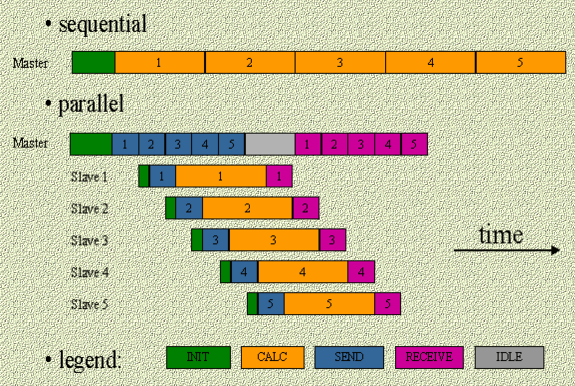
\includegraphics[scale=0.5]{SvsP.png}

This figure illustrates how the parallel approach will take a shorter period of time to convert images to thumbnails in large groups of data. If the groups of data are smaller, then the sequential approach may take a shorter period of time due to the fact that the benefits of parallel will show if and only if the collection of data is large enough.

%----------------------------------------------------------------------------------------
%	SECTION 3
%----------------------------------------------------------------------------------------
\section{A description of the challenges associated with performing experiments with image conversion.}
%Talk about the challenge of writting your own bash script and realizing that you have to make a bash script executable.
There were a number of challenges that arose with performing experiments with image conversion. One of the biggest challenges include writing your own bash script. I had decided to write my own bash script so I was able to perform all of the conversion approaches on a large data set of 499 images. In order to do so, I decided to write a bash script similar to the way the other download script files. When this occurs, it did not come to my attention for a while that when the bash script is written, it does not become executable. In order to do so, I had to write chmod +x, in order to make the bash script file executable.


%----------------------------------------------------------------------------------------
%	SECTION 4
%----------------------------------------------------------------------------------------

\section{A detailed paper that reports on the results arising from performing image conversion.}
\begin{lstlisting}
Cat
forloop.sh:
 0.290 seconds
 0.287 seconds
 0.407 seconds
 0.287 seconds
 0.285 seconds
 0.287 seconds
 0.551 seconds
 0.289 seconds
 0.289 seconds
 0.287 seconds
Mean(Average): 0.3259 seconds
Standard Deviation: 0.08755 

parallel.sh:
 0.400 seconds
 0.417 seconds
 0.408 seconds
 0.401 seconds
 0.409 seconds
 0.439 seconds
 0.404 seconds
 0.408 seconds
 0.416 seconds
 0.409 seconds
Mean(Average): 0.4111 seconds
Standard Deviation: 0.01126

xargs.sh:
 0.371 seconds
 0.330 seconds
 0.325 seconds
 0.329 seconds
 0.330 seconds
 0.328 seconds
 0.325 seconds
 0.329 seconds
 0.337 seconds
 0.326 seconds
Mean(Average): 0.333 seconds
Standard Deviation: 0.01379


Dog
forloop.sh:
 0.288 seconds
 0.285 seconds
 0.281 seconds
 0.286 seconds
 0.281 seconds
 0.276 seconds
 0.280 seconds
 0.286 seconds
 0.282 seconds
 0.281 seconds
Mean(Average): 0.2826 seconds
Standard Deviation: 0.0036

parallel.sh:
 0.401 seconds 
 0.405 seconds
 0.413 seconds
 0.415 seconds
 0.411 seconds
 0.400 seconds
 0.403 seconds
 0.388 seconds
 0.407 seconds
 0.412 seconds
Mean(Average): 0.4055 seconds
Standard Deviation: 0.00806

xargs.sh:
 0.346 seconds
 0.317 seconds
 0.329 seconds
 0.329 seconds
 0.323 seconds
 0.328 seconds
 0.328 seconds
 0.324 seconds
 0.330 seconds
 0.330 seconds
Mean(Average): 0.3285 seconds
Standard Deviation: 0.00741


Slides
forloop.sh:
 6.574 seconds
 5.297 seconds
 5.381 seconds
 5.346 seconds
 5.243 seconds
 5.281 seconds
 5.283 seconds
 5.263 seconds
 5.286 seconds
 5.305 seconds
Mean(Average): 5.4259 seconds
Standard Deviation: 0.40535

parallel.sh:
 2.885 seconds
 2.835 seconds
 2.800 seconds
 2.807 seconds
 2.812 seconds
 2.766 seconds
 2.833 seconds
 2.808 seconds
 2.762 seconds
 2.839 seconds
Mean(Average): 2.8147 seconds
Standard Deviation: 0.03614

xargs.sh:
 5.531 seconds
 5.368 seconds
 5.473 seconds
 5.419 seconds
 5.361 seconds
 5.379 seconds
 5.394 seconds
 5.409 seconds
 5.373 seconds
 5.336 seconds
Mean(Average): 5.4043 seconds
Standard Deviation:  0.05531


Cat, Dog, and Slides
forloop.sh:
 5.980 seconds
 5.983 seconds
 5.954 seconds
 5.920 seconds
 5.990 seconds
 5.992 seconds
 5.895 seconds
 5.903 seconds
 5.896 seconds
 5.822 seconds
Mean(Average): 5.4043 seconds
Standard Deviation: 0.0583

parallel.sh:
 3.304 seconds
 3.239 seconds
 3.392 seconds
 3.408 seconds
 3.328 seconds
 3.337 seconds
 3.283 seconds
 3.340 seconds
 3.283 seconds
 3.398 seconds
Mean(Average): 3.312 seconds
Standard Deviation: 0.05584

xargs.sh:
 6.190 seconds
 6.024 seconds
 6.054 seconds
 6.276 seconds
 6.043 seconds
 6.071 seconds
 6.039 seconds
 6.060 seconds
 5.978 seconds
 6.002 seconds
Mean(Average): 6.0737 seconds
Standard Deviation: 0.09065


Large Collection of 499 jpeg image
forloop.sh:
 7.402 seconds
 7.056 seconds
 7.209 seconds
 7.458 seconds
 7.008 seconds
 7.182 seconds
 7.009 seconds
 7.113 seconds
 7.251 seconds
 7.032 seconds
Mean(Average): 7.172 seconds
Standard Deviation: 0.1607

parallel.sh:
 5.813 seconds
 5.745 seconds
 5.771 seconds
 5.747 seconds
 5.677 seconds
 5.915 seconds
 5.846 seconds
 5.776 seconds
 5.798 seconds
 5.695 seconds
Mean(Average): 5.7783 seconds
Standard Deviation: 0.07009

xargs.sh:
 8.059 seconds
 8.064 seconds
 7.837 seconds
 7.871 seconds
 7.908 seconds
 7.460 seconds
 8.013 seconds
 8.087 seconds
 8.053 seconds
 7.989 seconds
Mean(Average): 7.9341 seconds
Standard Deviation: 0.188

\end{lstlisting}

%----------------------------------------------------------------------------------------
%	SECTION 5
%----------------------------------------------------------------------------------------
\section{A description of the challenges that you encountered when completing this assignment.}

There were a numnber of challenges that I had encountered when completing this assignment. One of these included to be able to complete this laboratory assignment using my MacBook Pro. In order to be able to complete the experiments that needed to be conducted for the completion of this laboratory assignment, I needed to install some packages. In order to do this, I decided to use homebrew. Homebrew is a package manager for Mac OS X. The packages that needed to be installed in order to complete this assignment using my MacBook Pro included ImageMagick and Parallel. Without the package ImageMagick installed, I would not have been able to convert any of the images. Without the package parallel, I would not have been able to run the parallel algorithm for any of the experiments.


%----------------------------------------------------------------------------------------
%	BIBLIOGRAPHY
%----------------------------------------------------------------------------------------

\nocite{Tange2011a}
\nocite{tanenbaum_steen_2007}
\nocite{mivule_2011}
\bibliographystyle{plain}

\bibliography{sample}

%----------------------------------------------------------------------------------------


\end{document}
